\chapter{Przedmiot pracy}

%\begin{itemize}
%  \item  Jak ja rozwiązuję problem?
%  \begin{itemize}
%    \item rozwiązanie zaproponowane przez dyplomanta
%    \item analiza teoretyczna rozwiązania
%    \item uzasadnienie wyboru zastosowanych metod, algorytmów, narzędzi
%  \end{itemize}
%\end{itemize}

% \section{Rozwiązanie zaproponowane przez dyplomanta}

\section{Rozwiązanie problemu wyszukiwania tekstu w pliku tekstowym}

Przed wyborem metody sprawdzającej należy wykonać heurystykę danych. Jest to 
wymagane, ponieważ wydajność algorytmu jest ściśle powiązana z danymi, które
będą przeszukiwane. Jeżeli większość analizowanych danych mają charakter
tekstowy, to lepszym rozwiązaniem będzie skorzystanie z ostatniego algorytmu BM
(rys. \ref{sch:algoBoyerMoore}), jednak w innym przypadku warto wykorzystać jeden z 
pozostałych.

\begin{figure}[ht]
    \centering
    \begin{lstlisting}
#!/usr/bin/env python3
import os
import subprocess
from collections import defaultdict
def get_mime_type(file_path):
    result = subprocess.run(['file', '--mime-type', file_path], 
    capture_output=True, text=True)
    return result.stdout.split(': ')[1].strip()
def get_file_size(file_path):
    try:
        return os.path.getsize(file_path)
    except Exception:
        return 0
def collect_mime_stats(start_path='.'):
    mime_stats = defaultdict(lambda: {'size': 0, 'count': 0})
    total_size = 0
    total_count = 0
    for root, _, files in os.walk(start_path):
        for file in files:
        file_path = os.path.join(root, file)
        mime_type = get_mime_type(file_path)
        size = get_file_size(file_path)
        
        mime_stats[mime_type]['size'] += size
        mime_stats[mime_type]['count'] += 1
        total_size += size
        total_count += 1
    return mime_stats, total_size, total_count
def format_size_kb(size_bytes):
    return f"{size_bytes / 1024:.2f}"
def main():
    mime_stats, total_size, total_count = collect_mime_stats()
    sorted_stats = sorted(mime_stats.items(), key=lambda x: x[1]['size'], reverse=True)
    format_str = "{:<45} {:>10} KB {:>8}"
    for mime_type, stats in sorted_stats:
        print(format_str.format(
            mime_type,
            format_size_kb(stats['size']),
            stats['count']
        ))
    print(format_str.format(
        "Total",
        format_size_kb(total_size),
        total_count
    ))
    \end{lstlisting}
    \caption{Program pozwalający na wyświetlenie ilości danych w formacie MIME}
    \label{fig:code:pythonMimeProgram}
\end{figure}

Przedstawiony program został stworzony do ustalenia typów plików w zbiorze 
rozpakowanych archiwów \ref{fig:code:pythonMimeProgram}. Na tym zbiorze testowano działanie poszczególnych algorytmów.
Ten zbiór jest mniejszy, aby ograniczyć wpływ czytania z dysku na wyniki badań. 
Porównano typ plików na podstawie identyfikatora formatu danych MIME. Pozwala
on na określenie, z jakim typem danych pracujemy, aby przeszukać dane.


\begin{table}[hb]
    \centering
    \begin{tabular}{lr}
        \hline
        \textbf{Typ MIME} & \textbf{Ilość} \\
        \hline
        image/jpeg & 5,303 \\
        text/html & 2,473 \\
        image/gif & 2,353 \\
        text/xml & 1,233 \\
        application/pdf & 656 \\
        application/postscript & 488 \\
        text/plain & 285 \\
        application/x-java-applet & 270 \\
        application/zip & 153 \\
        text/x-c & 134 \\
        application/gzip & 126 \\
        text/x-c++ & 121 \\
        text/csv & 64 \\
        application/octet-stream & 56 \\
        text/x-java & 49 \\
        application/x-rar & 34 \\
        application/x-tar & 9 \\
        application/x-dosexec & 3 \\
        application/msword & 3 \\
        text/x-diff & 2 \\
        inode/x-empty & 2 \\
        application/x-compress-ttcomp & 2 \\
        application/vnd.openxmlformats-officedocument.wordprocessingml.document & 2 \\
        application/vnd.ms-cab-compressed & 2 \\
        application/vnd.microsoft.portable-executable & 2 \\
        application/mac-binhex40 & 2 \\
        application/x-ms-ne-executable & 1 \\
        application/x-msaccess & 1 \\
        application/x-ace-compressed & 1 \\
        \hline
    \end{tabular}
    \caption{Dystrybucja w danych na podstawie typu plików MIME}
    \label{tabela:typyMIMEdataset}
\end{table}

Wykorzystanie kilku znanych algorytmów do przeszukiwania zawartości
tekstu i sprawdzenie, który z nich najlepiej sprawdza się pod względem prędkości
i dokładności wyszukiwania. Porównano ilość plików (tab. \ref{tabela:typyMIMEdataset}),
które występują w zbiorze danych i odrzucono część z nich z powodu sposobu, w jaki
analizowano dane.

Program nie ma na celu modyfikować informacji zawartych w plikach w żaden sposób.
Algorytmy użyte skupiają się głównie na tekście, dlatego w procesie tworzenia 
odrzucone zostają pliki z takimi rozszerzeniami jak:

\begin{enumerate}
  \item pliki zdjęć:
  \begin{itemize}
    \item ".jpg",  
    \item ".gif",
  \end{itemize}
  \item pliki skompresowane:
  \begin{itemize}
    \item ".tar.gz",
    \item ".tgz",
    \item ".gz",
  \end{itemize}
  \item pliki pochodzące od Microsoftu:
  \begin{itemize}
    \item ".doc", 
  \end{itemize}
\end{enumerate}

Innym sposobem na rozwiązanie problemu jest wykorzystanie dostępnych narzędzi i
dostosowanie ich do problemu, który jest rozwiązywany. Wykorzystanie wielu narzędzi
zaimplementowanych w jednym celu (\textbf{tar},\textbf{gzip}, \textbf{grep}) i połączenie ich do 
skomplikowanej operacji przeszukiwania archiwów zajełoby więcej czasu
i wymagałoby obsłużenia błędów każdego z narzędzi. Dodatkowo nie każda treść
jest odpowiednia do użycia narzędzia rozpakowującego tar, np. w przypadku 
skompresowanej treści, gdzie należy wykorzystać narzędzie \textbf{gzip}.

\section{Rozwiązanie problemu zarchiwizowanych plików w zbiorze danych}

Zbiór danych składa się danych zawierających archiwa oraz pliki skompresowane,
które zawierają drzewo innych plików skompresowanych i archiwów.
Aby odczytać wystąpienia, należy je rozpakować, jednak to powoduje ciągłe 
wydłużanie się ścieżki, a w Windows jest ona ograniczona do 256 znaków. Na 
systemie Linux ten limit nie powinien być problemem, gdyż system pozwala na 
ścieżki długości 4096 znaków, jednak ta różnica może wpływać na jakość działania
programu na różnych systemach.

Pliki zawierające archiwum zostaną rozpakowane do osobnego folderu, a następnie
wykonane zostanie rekurencyjne wyszukanie zawartość w każdym folderze i pliku.
Ta metoda zostanie powtórzona tak długo, aż wszystkie pliki zostaną odczytane 
i nie będzie już więcej archiwów do rozpakowania.

Aby porównać analizowane programy z implementacją gsearch, potrzeba porównać
ilość oczekiwanych rezultatów dla długości słów oraz czas wykonania całego 
przeszukania.

\section{Uzasadnienie wyboru zastosowanych metod, algorytmów, narzędzi}

\subsection{Użycie języka Golang}

Do utworzenia programu wykorzystam nowoczesny język programowania Golang \cite{bib:internet:golang}.
Posiada on bardzo wygodny model współbierzności programu co może okazać się 
kluczowe w przypadku tego rodzaju problemu. Dodatkowym plusem tego języka jest
to, że jego składnia jest bardzo czytelna i wzorująca na prostocie początkowych
kompilowanych języków programowania (C).

Zaletą Golang jest to, że jest kompilowany i tworzy się natywny dla danego 
systemu plik binarny. Daje to możliwość łatwego przenoszenia programu wynikowego.
Jest to też przewaga nad innymi językami programowania takimi jak python czy
javascript, gdyż te języki są interpretowane i z natury wolniejsze niż kod 
binarny. Golang nie wymaga dodatkowego poziomu abstrakcji w postaci maszyny 
wirtualnej czytającej bytecode jak w przypadku Javy i JVM.

\begin{figure}[h]
\centering
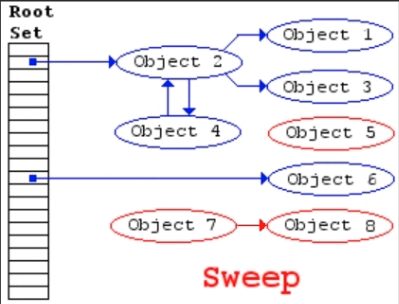
\includegraphics[width=0.5\textwidth]{./images/GarbageCollector.png}
\caption{Przykładowe działanie Garbage Collectora w programie}
\label{fig:GarbageCollectorImage}
\end{figure}
%https://upload.wikimedia.org/wikipedia/commons/4/4a/Animation_of_the_Naive_Mark_and_Sweep_Garbage_Collector_Algorithm.gif

Wadą tego języka może być fakt, iż język nie daje programiście możliwości pełnej
kontroli pamięci. Język wykorzystuje ang. \english{Garbage Collector} (zbieracz 
śmieci), który jest alternatywą do sposobu manualnej alokacji pamięci. Można 
zaobserwować działanie Garbage Collectora (GC) (rys. \ref{fig:GarbageCollectorImage}),
jak obiekty wykorzystywane w zbiorze korzenia (ang. \english{Root Set}) oznaczone na 
niebiesko, zostaną utrzymane w pamięci z powodu powiązania z innymi elementami
łączącymi się do zbioru korzenia. Kolorem czerwonym oznaczone są elementy, które
przestały być powiązane z jakimkolwiek elementem, więc zostaną zwolnienie z 
użycia, po zakończeniu operacji sprawdzania. 

GC wykorzystuje dwa warianty oznaczania danych. Pierwszy to tradycyjny sposób
skalarny, w którym każde wykorzystanie elementu w kodzie jest liczone i
zapisywane. W przypadku, gdy żaden fragment kodu nie wykorzystuje pamięci,
\english{Garbage Collector} uwalnia przydzieloną pamięć. Problem może skutkować
 wolniejszą egzekucją oraz pauzami w celu oczyszczenia pamięci.

Drugą metodą, która jest preferowana to warianty wektorowy, który wykorzystuje 
operacje SIMD, i dzięki temu może uwalniać większe ilości pamięci w mniejszej
ilości cykli. 

Kolejną zaletą jest to, że wewnętrznie Golang wykorzystuje większe obszary
przydzielonej pamięci. W przypadku, gdy program nie potrzebuje pamięci, program
wewnętrznie ją uwalnia, jednak nie oddaje jej od razu do systemu, jeżeli będzie 
ona wykorzystywana ponownie. Taki mechanizm zmniejsza częstotliwość operacji
systemowych, które wymagają potwierdzenia alokacji, zanim praca na pamięci 
zostanie wykonana. 

Program utworzony w ramach pracy porównuje różnicę pomiędzy sytuacją, w której
programista sam przydzielił pamięć i wykorzystywał ją ponownie do czytania 
zawartości plików oraz sytuacje, w której pozwolił kompilatorowi na własną
optymalizację alokowania bufora do odczytu plików.

\subsection{Użycie osobnej biblioteki do dearchiwizacji}

Do rozpakowania archiwów danych zastosowano bibliotekę unarr, które posiadała
dobrą dokumentację odpowiadającą zadaniu, które należało wykonać. Okazała się
problematyczna w stosunku niektórych archiwów.

\subsection{Rozpakowywanie plików na dysk zamiast w pamięci}

Zdecydowano się na rozpakowane danych w folderze tymczasowym. Próba 
rozpakowywania zawartości w pamięci powodowała uszkodzenie stosu z powodu zbyt
dużej ilości danych przechowywanych w pamięci przez Garbage Collector w języku Golang.


%%%%%%%%%%%%%%%%%%%%%%%%%%%%%%%%%%%%%%%%%%%%%%%%%%%%%%%%%%%%%%%%%%%%%%%%%%%%%%%%
%W całym dokumencie powinny znajdować się odniesienia do zawartych w nim ilustracji (rys. \ref{fig:2}).
%\begin{figure}
%\centering
%\begin{tikzpicture}
%\begin{axis}[
%    y tick label style={
%        /pgf/number format/.cd,
%            fixed,   % po zakomentowaniu os rzednych jest indeksowana wykladniczo
%            fixed zerofill, % 1.0 zamiast 1
%            precision=1,
%        /tikz/.cd
%    },
%    x tick label style={
%        /pgf/number format/.cd,
%            fixed,
%            fixed zerofill,
%            precision=2,
%        /tikz/.cd
%    }
%]
%\addplot [domain=0.0:0.1] {rnd};
%\end{axis} 
%\end{tikzpicture}
%\caption{Wykres przebiegu funkcji.} % Podpis jest zawsze POD rysunkiem.
%\label{fig:2}
%\end{figure}


%%%%%%%%%%%%%%%%%%%%%
%% RYSUNEK Z PLIKU
%
%\begin{figure}
%\centering
%
\includegraphics[width=0.5\textwidth]{./graf/politechnika_sl_logo_bw_pion_pl.pdf}
%\caption{Podpis rysunku zawsze pod rysunkiem.}
%\label{fig:etykieta-rysunku}
%\end{figure}
%Rys. \ref{fig:etykieta-rysunku} przestawia …
%%%%%%%%%%%%%%%%%%%%%
%
%%%%%%%%%%%%%%%%%%%%%
%% WIELE RYSUNKÓW 
%
%\begin{figure}
%\centering
%\begin{subfigure}{0.4\textwidth}
%    
\includegraphics[width=\textwidth]{./graf/politechnika_sl_logo_bw_pion_pl.pdf}
%    \caption{Lewy górny rysunek.}
%    \label{fig:lewy-gorny}
%\end{subfigure}
%\hfill
%\begin{subfigure}{0.4\textwidth}
%    
\includegraphics[width=\textwidth]{./graf/politechnika_sl_logo_bw_pion_pl.pdf}
%    \caption{Prawy górny rysunek.}
%    \label{fig:prawy-gorny}
%\end{subfigure}
%
%\begin{subfigure}{0.4\textwidth}
%    
\includegraphics[width=\textwidth]{./graf/politechnika_sl_logo_bw_pion_pl.pdf}
%    \caption{Lewy dolny rysunek.}
%    \label{fig:lewy-dolny}
%\end{subfigure}
%\hfill
%\begin{subfigure}{0.4\textwidth}
%    
\includegraphics[width=\textwidth]{./graf/politechnika_sl_logo_bw_pion_pl.pdf}
%    \caption{Prawy dolny rysunek.}
%    \label{fig:prawy-dolny}
%\end{subfigure}
%        
%\caption{Wspólny podpis kilku rysunków.}
%\label{fig:wiele-rysunkow}
%\end{figure}
%Rys. \ref{fig:wiele-rysunkow} przestawia wiele ważnych informacji, np. rys. \ref{fig:prawy-gorny} jest na prawo u góry.
%%%%%%%%%%%%%%%%%%%%%


%Tekst dokumentu powinien również zawierać odniesienia do tabel (tab. \ref{id:tab:wyniki}).
%\begin{table}
%\centering
%\caption{Opis tabeli nad nią.}
%\label{id:tab:wyniki}
%\begin{tabular}{rrrrrrrr}
%\toprule
%	         &                                     \multicolumn{7}{c}{metoda}                                      \\
%	         \cmidrule{2-8}
%	         &         &         &        \multicolumn{3}{c}{alg. 3}        & \multicolumn{2}{c}{alg. 4, $\gamma = 2$} \\
%	         \cmidrule(r){4-6}\cmidrule(r){7-8}
%	$\zeta$ &     alg. 1 &   alg. 2 & $\alpha= 1.5$ & $\alpha= 2$ & $\alpha= 3$ &   $\beta = 0.1$  &   $\beta = -0.1$ \\
%\midrule
%	       0 &  8.3250 & 1.45305 &       7.5791 &    14.8517 &    20.0028 & 1.16396 &                       1.1365 \\
%	       5 &  0.6111 & 2.27126 &       6.9952 &    13.8560 &    18.6064 & 1.18659 &                       1.1630 \\
%	      10 & 11.6126 & 2.69218 &       6.2520 &    12.5202 &    16.8278 & 1.23180 &                       1.2045 \\
%	      15 &  0.5665 & 2.95046 &       5.7753 &    11.4588 &    15.4837 & 1.25131 &                       1.2614 \\
%	      20 & 15.8728 & 3.07225 &       5.3071 &    10.3935 &    13.8738 & 1.25307 &                       1.2217 \\
%	      25 &  0.9791 & 3.19034 &       5.4575 &     9.9533 &    13.0721 & 1.27104 &                       1.2640 \\
%	      30 &  2.0228 & 3.27474 &       5.7461 &     9.7164 &    12.2637 & 1.33404 &                       1.3209 \\
%	      35 & 13.4210 & 3.36086 &       6.6735 &    10.0442 &    12.0270 & 1.35385 &                       1.3059 \\
%	      40 & 13.2226 & 3.36420 &       7.7248 &    10.4495 &    12.0379 & 1.34919 &                       1.2768 \\
%	      45 & 12.8445 & 3.47436 &       8.5539 &    10.8552 &    12.2773 & 1.42303 &                       1.4362 \\
%	      50 & 12.9245 & 3.58228 &       9.2702 &    11.2183 &    12.3990 & 1.40922 &                       1.3724 \\
%\bottomrule
%\end{tabular}
%\end{table}  

